\chapter{REVISÃO DE LITERATURA}\label{chap:fundamentacaoTeorica}

Para o presente trabalho, em decorrência dos instrumentos e sensores escolhidos, devemos colher na literatura as equações e formalismos que descrevem o movimento e a orientação dos corpos no espaço, bem como as relações com as forças envolvidas. Além da literatura básica sobre mecânica~\cite{Goldstein1980}, robótica ~\cite{Craig2014} e controle ~\cite{Ogata2010}, os temas são mais bem explorados na literatura sobre controle de aeronaves e mísseis~\cite{Henderson1997}, \cite{Stevens2016}, \cite{Blakelock1991} ou sobre navegação inercial~\cite{Stovall1997}, \cite{Weston2004}, \cite{Wang2021} e~\cite{Haoran2019}.

No particular, empregaremos em grande parte as convenções e equações utilizadas em~\cite{Stevens2016}, que acreditamos dar um tratamento mais direto e acessível a esses temas.

\section{Notação e convenções}

Neste trabalho utilizamos um modelo de mundo tridimensional e mecânica clássica.  Nosso espaço é estruturado por três eixos ortogonais \(x\), \(y\), \(z\) (\(1, 2, 3\)) onde uma posição é dada por um vetor tridimensional. Descreveremos a atitude e o movimento de um corpo rígido sobre a superfície oblata e girante da Terra. Não obstante, serão empregadas aproximações sobre uma pequena área para um plano tangente à Terra estacionária e constante, que basta\footnotemark{} para os nossos propósitos. Para simbologia, acompanhamos~\cite{Stevens2016}:

\begin{align*}
    \mathbf{p}_{A/B} &\equiv
    \text{ vetor posição do ponto A em relação ao ponto B} \\
    \mathbf{v}_{A/i} &\equiv
    \text{ vetor velocidade do ponto \(A\) tomada no sistema \(F_{i}\)} \\
    ^{b}\mathbf{\dot{v}}_{A/i} &\equiv
    \text{ vetor derivada de \(\mathbf{v}_{A/i}\) tomada no sistema \( F_{b}\)} \\
    \mathbf{v}^{c}_{A/i} &\equiv \left( \mathbf{v}_{A/i} \right)^{c} \equiv
    \text{ conjunto dos componentes de \(\mathbf{v}_{A/i}\) expressos no sistema \(c\)} \\
\end{align*}

Componentes de vetores terão índices para indicar o sistema de coordenadas ou serão denotados pelo símbolo de vetor com índices \(x\), \(y\), e \(z\) para indicar as coordenadas, exceto quando indicado pelo símbolo transposto, e todos vetores são do tipo vetor coluna. Acompanhando~\cite{Stevens2016}, por exemplo:
\begin{align*}
    &\mathbf{p}^{b}_{A/B} = \begin{bmatrix}x_{b} \\ y_{b} \\ z_{b}\end{bmatrix}&
    \text{ ou }&
    &\mathbf{v}^{b}_{A/i} = \begin{bmatrix} v_{x} \\ v_{y} \\ v_{z} \end{bmatrix} = \begin{bmatrix} v_{x} & v_{y} & v_{z} \end{bmatrix}^{T}
\end{align*}

\footnotetext{A título de advertência, o assunto não é simples, com diversos formalismos possíveis, um campo fértil para confusão. Por exemplo, a atitude de um corpo pode ser descrita em três dimensões com ângulos de Euler ao menos em doze sequências de rotações anti-horárias distintas, não intercambiáveis, ou ainda pode ser descrita em quatro dimensões com o uso do quaternion, conforme observamos em~\cite{Henderson1997}. Além disso, é importante separar a orientação relativa do nosso espaço tridimensional em abstrato, do eixo de referência em relação ao nosso espaço abstrato, e do sistema móvel que pretendemos descrever em relação ao sistema de referência. No presente trabalho adotaremos um único formalismo que atende aos nossos propósitos limitados, e remetemos o leitor às fontes para aprofundamento do assunto.}

\section{Descrevendo a atitude de um corpo}

Descrevemos a atitude de um robô em ângulos de Euler na sequência \(z\), \(y\), \(x\) (3, 2, 1) que leva de um sistema de referência fixo na Terra até um sistema fixo no corpo do robô. Escolhemos o sistema (\(ned\)) - ``North-East-Down'' (Norte, Leste, Abaixo) com o eixo \(x\) apontando para o Norte, o eixo \(z\) Abaixo, o eixo \(y\) completando o sistema de coordenadas, e o sistema (\(frd\)) - ``Front-Right-Down'' (Avante, Direita, Abaixo), fixo no robô, com eixos, respectivamente, (\(x\),\(y\),\(z\)), sendo o Avante alinhado à \emph{linha de referência longitudinal} do robô, com ``Avante'' e ``Abaixo'' situados no plano de simetria, e o eixo Direito completando o sistema. Adotamos, ainda a convenção de rotações anti-horárias (regra da mão direita).

Desse a modo, a sequência de rotações que leva do sistema de referência \(ned\) para o sistema \(frd\) no corpo é dada por:
\begin{enumerate}
    \item Rotação anti-horária sobre eixo \(z\), ou \(\psi\) positivo (\textit{``compass heading''})
    \item Rotação anti-horária sobre novo eixo \(y'\), ou \(\theta\) positivo (\textit{pitch})
    \item Rotação anti-horária sobre novo eixo \(x''\), ou \(\phi\) positivo (\textit{roll})
\end{enumerate}

Esta sequência de rotações é normalmente denominada \emph{``yaw, pitch, roll''} (guinada, arfada e rolagem), partindo do sistema de referência.

Podemos escrever as matrizes de rotação abreviando co-seno por \(c\) e seno por \(s\). Esta matriz representa uma transformação padrão que será utilizada ao longo do texto, acompanhando~\cite{Stevens2016}:

\begin{align*}
    C_{f\!r\!d\!/\!n\!e\!d} =
    \begin{bmatrix}
        1               &  0            &  0             \\
        0               &  \cos{\phi}   &  \sin{\phi}    \\
        0               & -\sin{\phi}   &  \cos{\phi}
    \end{bmatrix}
    \begin{bmatrix}
        \cos{ \theta}   &  0            & -\sin{\theta} \\
        0               &  1            &  0            \\
        \sin{ \theta}   &  0            &  \cos{\theta}
    \end{bmatrix}
    \begin{bmatrix}
        \cos{\psi}      &  \sin{\psi}   &  0             \\
       -\sin{\psi}      &  \cos{\psi}   &  0             \\
        0               &  0            &  1
    \end{bmatrix}
\end{align*}
\begin{align}\label{eq:matrix-yaw-pitch-roll} %\tag{1.3-10}
    C_{f\!r\!d\!/\!n\!e\!d} &=
    \begin{bmatrix}
        c\theta c\psi   & c\theta s\psi & -s\theta    \\
        \left(-c\phi s\psi + s\phi s\theta c\psi \right)
        &  \left( c\phi c\psi + s\phi s\theta s\psi \right)
        &  s\phi c\theta                                 \\
        \left( s\phi s\psi + c\phi s\theta c\psi \right)
        &  \left( -s\phi c\psi + c\phi s\theta s\psi \right)
        & c\phi c\theta
    \end{bmatrix}
\end{align}

O intervalo de validade para o qual os ângulos de rotação são bem definidos\footnotemark{} é:
\begin{align*}
    -\pi  < \phi \leq \pi \\
    -\frac{\pi}{2} \leq \theta \leq \frac{\pi}{2} \\
    -\pi < \psi \leq \pi
\end{align*}

\footnotetext{A título de exemplo, ponderamos que caso o ângulo \( \theta \) fosse definido no intervalo de \( \pm 180^{\circ} \) o veículo estaria apontando para o Sul com os ângulos \(\phi\) e \(\psi\) em \( 0^{\circ}\) o que é indesejável pois pode confundir a interpretação.}

\section{Cinemática Rotacional}

Aqui definiremos a derivada de um vetor, mostraremos como ela depende do sistema de referência do observador, e relacionamos as derivadas de um vetor, tomadas em dois sistemas de referência distintos, através do vetor velocidade angular relativa entre esses dois sistemas.

Genericamente a derivada de um vetor é similar à de um escalar~\cite{Stevens2016}:
\begin{equation*}
    \frac{\mathrm{d}}{\mathrm{d}t} \mathbf{p}_{A/B} =  \lim_{\delta t \rightarrow 0 } \begin{bmatrix}
        \displaystyle\frac{\mathbf{p}_{A/B} (t + \delta t) - \mathbf{p}_{A/B} (t) }{\delta t}
    \end{bmatrix}
\end{equation*}

Este novo vetor decorre das mudanças de módulo e orientação de \(\mathbf{p}_{A/B}\). Sendo \(\mathbf{p}\) um vetor livre (por exemplo, a velocidade) sua derivada independe de sua posição, e as mudanças de comprimento e direção decorram do movimento da ponta de \(\mathbf{p}\) em relação à própria cauda. Seja \(\mathbf{p}\) seja um vetor vinculado a algum sistema (por exemplo, o vetor posição) sua derivada naquele sistema é um vetor livre que corresponde à ponta de \(\mathbf{p}\).

\subsection{Velocidade Angular como Vetor}

Um vetor pode apontar em qualquer direção por meio de uma simples rotação ao longo de um eixo apropriado. A fórmula para essa rotação é descrita em~\cite{Goldstein1980}:

\begin{figure}[h]
    \centering
    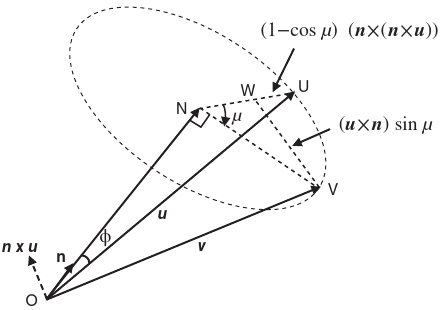
\includegraphics[width=0.5\textwidth, keepaspectratio]{figuras/figure1.2-1.png}\label{fig1.2-1}
    \caption{Rotação de um vetor}\label{fig:rotacao-de-um-vetor}
    \fonte{\cite{Goldstein1980}}
\end{figure}

Na figura acima, o vetor \(\mathbf{u}\) foi rotacionado para formar o vetor \(\mathbf{v}\) ao definirmos um eixo de rotação ao longo do vetor \(\mathbf{n}\) e realizarmos uma rotação pelo ângulo \(\mu\) ao redor de \(\mathbf{n}\). Estes dois vetores se somam a \(\mathbf{u}\) para obtermos \(\mathbf{v}\), e obtemos:
    \begin{align}
        \mathbf{v} &= \mathbf{u} + \left(1 - {\cos{\mu}}\right) \left(\mathbf{n}\!\times\!\left(\mathbf{n}\!\times\!\mathbf{u}\right)\right) - \left(\mathbf{n}\!\times\!\mathbf{u}\right){\sin{\mu}}\label{eq:rotation-formula-a} %\tag{1.2-5a}
    \end{align}
    \begin{align}
        \mathbf{v} = \left(1 - {\cos{\mu}}\right) \mathbf{n}\!\left(\mathbf{n}\cdot\mathbf{u}\right) + \mathbf{u}{\cos{\mu}} - \left(\mathbf{n}\!\times\!\mathbf{u}\right){\sin{\mu}} \label{eq:rotation-formula-b}  % \tag{1.2-5b}
    \end{align}

    As equações acima (\ref{eq:rotation-formula-a} e~\ref{eq:rotation-formula-b}), às vezes chamadas de \textit{fórmula de rotação}, nos mostram que definindo \(\mathbf{n}\) e \(\mu\) podemos operar sobre \(\mathbf{u}\) com produtos escalares e vetoriais para obter a rotação desejada, independente de sistemas de coordenadas ou magnitude do ângulo.

    Partindo da figura acima, fazemos uma rotação muito pequena \(\delta\mu \ll 1 \text{rad}\), definindo \(\mathbf{v} = \mathbf{u} + \delta \mathbf{u}\), e, aplicando a equação (\ref{eq:rotation-formula-a}) obtemos:
\begin{equation*}
    \delta \mathbf{u} \approx -\!\sin(-\delta\mu)\mathbf{n}\!\times\!\mathbf{u} \approx (\mathbf{n}\!\times\!\mathbf{u})\delta\mu
\end{equation*}

Dividindo por \(\delta t\), no limite onde \(\delta t \rightarrow 0\), definindo \(\mathbf{\omega} \equiv \dot{\mu}\mathbf{n}\), obtemos:

\begin{equation}
    \dot{\mathbf{u}} = \mathbf{\omega}\!\times\!\mathbf{u}\label{eq:vector-derivative} %\tag{1.4-1}
\end{equation}

Esta equação relaciona a velocidade translacional da ponta do vetor \(\mathbf{u}\) ao vetor \(\mathbf{\omega}\). Este vetor \(\mathbf{\omega}\), que denominados \textit{vetor velocidade angular}, constitui-se de um vetor unitário  que define o eixo de rotação, multiplicado pela taxa de rotação. Este é um vetor livre, pode ser transladado paralelo a si mesmo, e axial, que mudaria de direção caso houvéssemos escolhido uma convenção de sentido horário para a rotação.

Dessa forma podemos associar \(\mathbf{\omega}\) ao sistema de coordenadas fixado no corpo, atribuindo índices, para representar a velocidade angular do corpo em relação a outro determinado sistema.

Como vimos, a atitude de um corpo rígido pode ser descrita por uma matriz rotacional variante no tempo, e, pelo teorema de Euler\footnotemark{}, esse corpo possui um único \emph{eixo instantâneo de rotação} ao qual o vetor velocidade angular é paralelo, também único.

\footnotetext{\emph{``Euler's Theorem: The general displacement of a rigid body with one point fixed is a rotation about some axis.''} Para uma explicação a respeito, vide~\cite{Goldstein1980}, Capítulo 4.}

\section{Cinemática e Ângulos de Euler}

Um corpo em movimento pode mudar sua atitude, descrita em ângulos de Euler, ao longo do tempo, e, neste sentido, podemos falar de uma taxa de mudança de cada um desses ângulos de Euler ao longo do tempo. Essas taxas são coisa distintas, é preciso dizer, do vetor velocidade angular do corpo.

Para vincular as taxas de ângulos de Euler, que descrevem a mudança de atitude de um corpo, à sua velocidade angular, procedemos do seguinte modo. Definimos um quadro de referência \(F_{r}\) e um quadro do corpo \(F_{b}\) com vetor velocidade angular relativa \(\omega_{b/r}\) e uma sequencia de ângulos de Euler que define a atitude do corpo, ou seja, a orientação do sistema de coordenadas preso ao corpo em relação ao sistema de referência. Cada taxa de ângulos de Euler informa a direção e magnitude para um determinado vetor velocidade angular sobre um eixo de coordenadas em particular. Esses três vetores somados formam o vetor velocidade angular resultante do veículo cujas taxas de ângulos de Euler estamos tratando. Desse modo podemos encontrar os componentes do vetor velocidade angular resultante \cite{Stevens2016}.

Em outras palavras, movemos sobre a Terra um sistema de coordenada \(frd\) (\emph{``front'', ``right'', ``down''} - frente, direita, abaixo) preso no corpo, com o sistema \(ned\) (\emph{``north'', ``east'', ``down''} - norte, leste abaixo) fixo no quadro de referência, usando uma sequencia ``yaw-pitch-roll'' de ângulos de Euler do sistema \(ned\) para o sistema \(frd\). No caso das equações de plano tangente o sistema \(ned\) é fixado na Terra, e a velocidade angular relativa é aquela do corpo em relação à Terra. Não trataremos aqui do caso mais geral das equações com seis graus de liberdade onde sistema \(ned\) se move sobre a Terra.

As transformações de coordenadas são~\cite{Stevens2016}:

\begin{align*}
    \mathbf{\omega}^{frd}_{b/r} = \begin{bmatrix} \dot\phi \\ 0 \\0 \end{bmatrix}
    + C_{\phi} \begin{pmatrix}
        \begin{bmatrix} 0 \\ \dot\theta \\ 0 \end{bmatrix}
        + C_{\theta}\begin{bmatrix} 0 \\ 0 \\ \dot\psi \end{bmatrix}
    \end{pmatrix}
\end{align*}

\ldots sendo \(C_{\phi}\) e \(C_{\theta}\)  as rotações (anti-horárias) dos planos por cada ângulo de Euler em particular, conforme equação (\ref{eq:matrix-yaw-pitch-roll}). Multiplicando as matrizes, teremos:

\begin{align}\label{eq:1.4-3}% \tag{1.4-3}
    \mathbf{\omega}^{frd}_{b/r} \equiv \begin{bmatrix} P \\ Q \\ R \end{bmatrix}
    = \begin{bmatrix}
        1 & 0 & -\sin{\theta} \\
        0 & \cos{\phi} & \sin{\phi}\cos{\theta} \\
        0 & -\sin{\phi} & \cos{\phi}\cos{\theta}
    \end{bmatrix}
    \begin{bmatrix}
        \dot\phi \\
        \dot\theta \\
        \dot\psi
    \end{bmatrix}
\end{align}

\ldots sendo \(P\), \(Q\), \(R\), os componentes do vetor velocidade angular do corpo expressos no sistema \(frd\), respectivamente, rolagem (\emph{``roll''}), arfada (\emph{``pitch''}) e guinada (\emph{``yaw''}). A transformação inversa é dada por:

\begin{align}\label{eq:1.4-4}% \tag{1.4-4}
    \begin{bmatrix}
        \dot\phi \\
        \dot\theta \\
        \dot\psi
    \end{bmatrix}
    =
    \begin{bmatrix}
        1 & \sin{\phi}\tan{\theta} & \cos{\phi}\tan{\theta} \\
        0 & \cos{\phi} & -\sin{\phi} \\
        0 & \frac{\sin{\phi}}{\cos{\theta}} & \frac{\cos{\phi}}{\cos{\theta}}
    \end{bmatrix}
    \begin{bmatrix}
        P \\ Q \\ R
    \end{bmatrix}
\end{align}

Para simplificar, definimos \(\mathbf{\Phi} \equiv \left[\phi \theta \psi \right]^T \) e reescrevemos  (\ref{eq:1.4-4}) assim:

\begin{equation}\label{eq:1.4-5}% \tag{1.4-5}
    \dot{\mathbf{\Phi}} = H \left( \mathbf{\Phi} \right) \mathbf{\omega}^{frd}_{b/r}
\end{equation}

As equações (\ref{eq:1.4-3}) e (\ref{eq:1.4-4}) serão referidas como as equações cinemáticas de Euler, como faz~\cite{Stevens2016}. Note que as matrizes de coeficientes \emph{não são} matrizes ortogonais representando rotações ordinárias de coordenadas. Note ainda que as Equações (\ref{eq:1.4-4}) e (\ref{eq:1.4-5}) possuem uma singularidade quando  \(\theta = \pm \frac{\pi}{2}\). Ainda, se essas equações forem utilizadas em uma simulação, as taxas de ângulos de Euler podem integrar para ângulos fora do intervalos de ângulos de Euler, e portanto, seria necessário incluir uma lógica para lidar com essa situação no programa simulador. Não obstante, as equações cinemáticas de Euler são bastante empregadas em simulações.

\section{Derivada de um vetor em sistemas móveis}

Nesta seção deveremos obter as equações gerais para o movimento de um corpo no espaço tridimensional. Para generalizar a derivada de um vetor em relação em sistemas móveis obteremos \(^{a}\dot{\mathbf{p}}\) a partir da figura abaixo:
\begin{figure}[H]
    \centering
    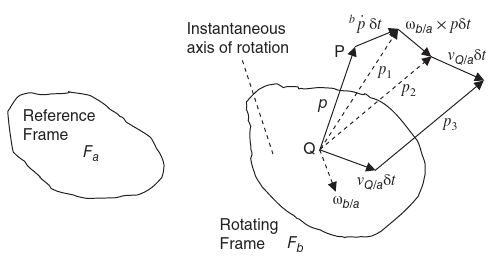
\includegraphics[width=0.5\textwidth, keepaspectratio]{figuras/figure1.4-1.png}\label{fig1.4-1}
    \caption{Derivada de um vetor em sistemas móveis.}
    \fonte{\cite{Stevens2016}}
\end{figure}

Os sistemas \(F_{b}\) e \(F_{a}\) têm velocidade angular relativa \(\mathbf{\omega}_{b/a}\). O ponto \(Q\), fixo em \(F_{b}\), traslada em relação a \(F_{a}\) a uma velocidade \(\mathbf{v}_{Q/a}\). Partindo de  \(Q\) nasce o vetor \(\mathbf{p}\). Observando a partir de \(F_{b}\) estabelecemos \(\mathbf{p}_{1}\) ao acrescentar o efeito \({^b\dot{\mathbf{p}}}\). Olhando a partir de \(F_{a}\) estabelecemos o vetor  \(\mathbf{p}_{2}\) ao somar, ainda, o efeito de \(\mathbf{\omega}_{b/a}\). A partir de \(F_{a}\), estabelecemos \(\mathbf{p}_{3}\) somando o efeito de \(\mathbf{v}_{Q/a}\), que, entretanto, não muda o comprimento ou direção de \(\mathbf{p}_{2}\).Portanto, para obtermos \(^{a}\dot{\mathbf{p}}\) devemos  comparar \(\mathbf{p}_{2}\) a \(\mathbf{p}\) quando \(\delta t \rightarrow 0\). Desse modo, no instante \(\delta t\), \(\mathbf{p}_{2} \!-\! \mathbf{p}\) temos:
\begin{equation*}
    \mathbf{p}_{2} - \mathbf{p} = {^{b}\dot{\mathbf{p}}} \delta t + \left( \mathbf{\omega}_{b/a} \! \times \!\mathbf{p} \right) \delta t
\end{equation*}

Dividindo por \(\delta t\) no limite em que \(\delta t \rightarrow 0\) resulta na equação\footnotemark{}:
\begin{equation} \label{eq:1.4-2}
    {^{a}\dot{\mathbf{p}}} = {^{b}\dot{\mathbf{p}}} + {\mathbf{\omega}_{b/a} \! \times \!\mathbf{p}}
\end{equation}

\footnotetext{Conhecida por ``Equação de Coriolis''~\cite{Stevens2016},~\cite{Blakelock1991}.}

Dentre as propriedades do vetor velocidade angular destacamos\footnotemark{}:
\begin{enumerate}[label=\alph*)]
\item É único e relaciona as derivadas de um vetor tomadas em dois sistemas.
\item Satisfaz a condição de movimento relativo \(\mathbf{\omega}_{b/a} = - \mathbf{\omega}_{a/b}\).
\item É aditivo entre sistemas, ou seja, \(\mathbf{\omega}_{c/a} = \!\mathbf{\omega}_{c/b} + \mathbf{\omega}_{b/a}\) (não vale para aceleração angular).
\item A derivada é equivalente em ambos os sistemas: \({^{a}\dot{\mathbf{\omega}}_{b/a}} = {^{b}\dot{\mathbf{\omega}}_{a/b}} \).
\end{enumerate}
\footnotetext{Seguindo~\cite{Stevens2016}}.

Ainda, derivada de um vetor em um quadro pode ser encontrada a partir das derivadas dos seus componentes expressas em um sistema fixo no mesmo quadro, por exemplo:
\begin{equation*}
    \mathbf{v}^{a\!f} = \begin{bmatrix} v_{x} & v_{y} & v_{z} \end{bmatrix}^{T}
\end{equation*}

\section{Velocidade e Aceleração em quadros móveis}

Encontraremos velocidade e aceleração do ponto \(P\), situado em \(\mathbf{p}\), que se move em relação a \(F_{a}\) e \(F_{b}\), onde fixamos~\(O\)~e~\(Q\), respectivamente, os quais também se movem em relação um ao outro. Na figura abaixo, relacionamos os vetores posição, tomamos suas derivadas no quadro de referência\footnotemark{} \(F_{a}\),  determinando a velocidade. Usando \(\mathbf{v}\) para um vetor velocidade, aplicamos a equação de Coriolis obtendo~\cite{Stevens2016}:
\footnotetext{A escolha do quadro \(F_{a}\) como referência é arbitrária.}
\begin{figure}[H]
    \centering
    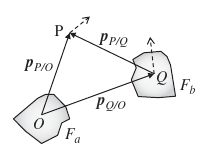
\includegraphics[width=0.25\textwidth, keepaspectratio]{figuras/figure1.5-1.png}\label{fig1.5-1}
    \caption{Velocidade e aceleração em quadros móveis}
    \fonte{\cite{Stevens2016}}
\end{figure}
\begin{align}
    \mathbf{p}_{P/O}             &= \mathbf{p}_{Q/O} + \mathbf{p}_{P/Q} \label{eq:1.5-1} \\
    {^{a}\dot{\mathbf{p}}_{P/O}} &= {^{a}\dot{\mathbf{p}}_{Q/O}} + {^{a}\dot{\mathbf{p}}_{P/Q}} \label{eq:1.5-2} \\
    \mathbf{v}_{P/a}             &= \mathbf{v}_{Q/a} + \left( \mathbf{v}_{P/b} + \mathbf{\omega}_{b/a}\!\times\!\mathbf{p}_{P/Q} \right) \label{eq:1.5-3}
\end{align}

Rearranjando para destacar os termos em parênteses\footnotemark{}:
\begin{equation*}
    \mathbf{v}_{P/a} = \mathbf{v}_{P/b} + \left( \mathbf{v}_{Q/a} + \mathbf{\omega}_{b/a}\!\times\!\mathbf{p}_{P/Q} \right),
\end{equation*}
\footnotetext{O termo em parênteses corresponde à chamada \textit{velocidade de transporte de \(P\) no quadro \(F_{a}\)} (a velocidade em \(F_{a}\) de um ponto fixo em \(F_{b}\) coincidente com \(P\)).}

Para a aceleração derivamos (\ref{eq:1.5-3}) em \(F_{a}\). Velocidades em \(F_{a}\) se tornam acelerações em \(F_{a}\); A velocidade em \(F_{b}\) é derivada pela Equação de Coriolis; A produto vetorial é derivado pela ``regra do produto vetorial''; A derivada da velocidade angular é um vetor aceleração angular designado \(\mathbf{\alpha}\). Seja \(\mathbf{a}\) a aceleração translacional em (\ref{eq:1.5-3}), obtemos:
\begin{equation*}
    \mathbf{a}_{P/a} = \mathbf{a}_{Q/a} + \left(\mathbf{a}_{P/b} + \mathbf{\omega}_{b/a}\!\times\!\mathbf{v}_{P/b}\right) + {{\mathbf{\alpha}_{b/a}}\!\times\!{\mathbf{p}_{P/Q}}} + {\mathbf{\omega}_{b/a}}\!\times\!{\left({\mathbf{v}_{P/b}} + {{\mathbf{\omega}_{b/a}}\!\times\!{\mathbf{p}_{P/Q}}}\right)}
\end{equation*}

Reorganizando, destacamos aceleração ``\emph{de transporte}'', ``\emph{centrípeta}'' e ``\emph{de Coriolis}'':
\begin{equation}
    \mathbf{a}_{P/a} = \mathbf{a}_{P/b} + \overbrace{\mathbf{a}_{Q/a} + {{\mathbf{\alpha}_{b/a}}\!\times\!{\mathbf{p}_{P/Q}}} + \underbrace{{{\mathbf{\omega}_{b/a}}\!\times\!{\left({\mathbf{\omega}_{b/a}}\!\times\!{\mathbf{p}_{P/Q}}\right)}}}_{\text{aceleração centrípeta}}}^{\text{aceleração de transporte}} + \underbrace{{2\mathbf{\omega}_{b/a}\!\times\!\mathbf{v}_{P/b}}}_{\text{aceleração de Coriolis}} \label{eq:1.5-4}
\end{equation}


Os termos \({^{a}\mathbf{a}}\) e \({^{b}\mathbf{a}}\), denominados \emph{aceleração total} e \emph{aceleração relativa}, são expressos nos quadros de referência e secundário, respectivamente. Notamos o surgimento do termo \textit{aceleração de Coriolis}, a ser examinado mais adiante. Se fixamos \(P\) no quadro \(F_{b}\), nos resta apenas \textit{aceleração de  transporte}, definida como a aceleração expressa em \(F_{a}\) de um ponto fixo em \(F_{b}\) instantaneamente coincidente com \(P\). A aceleração de transporte expressa os efeitos do movimento de \(F_{b}\), em termos de aceleração do ponto \(Q\), da velocidade angular e da aceleração angular do quadro~\cite{Stevens2016}.


Por exemplo, um acelerômetro fixo num robô móvel, de corpo rígido, não se move em relação ao quadro do corpo do robô, restando apenas os termos relativos à velocidade e aceleração de transporte nas equações~(\ref{eq:1.5-3}) e~(\ref{eq:1.5-4}), respectivamente. A aceleração para o sensor no ponto \(P\), de posição \(\mathbf{p}_{P/Q}\) em relação ao ponto \(Q\) fixo no quadro do robô, denotando~\(a\)~e~\(b\) os quadros de referência e do robô, respectivamente, é dada por \cite{Stevens2016}:
\begin{equation*}
    {\mathbf{a}_{P/a}} = {\mathbf{a}_{Q/a}} + {\mathbf{\alpha}_{b/a}}\!\times\!{\mathbf{p}_{P/Q}} + {\mathbf{\omega}_{b/a}}\!\times\!\left({\mathbf{\omega}_{b/a}}\!\times\!{\mathbf{p}_{P/Q}}\right)
\end{equation*}

Aplicando para um corpo sobre a Terra, sejam \(F_{i}\)  e  \(F_{e}\) quadros de referencia inercial e fixo na Terra, respectivamente, e pontos \(Q\) e \(O\) coincidentes no centro de massa da Terra (sem aceleração translacional), o \(\mathbf{p}_{P/Q}\) é um vetor posição geocêntrico, e \(\mathbf{a}_{Q/a}=0\). Considerando que a Terra gira a uma velocidade angular constante, a derivada de \(\mathbf{\omega}_{b/a}\) também desaparece. Restam a aceleração relativa, a centrípeta e a de Coriolis na equação que relaciona a aceleração verdadeira (inercial) à aceleração relativa, para aplicar as leis de Newton no movimento de um ponto \(P\) sobre a Terra~\cite{Stevens2016}:
\begin{equation} \label{eq:1.5-5}
    {\mathbf{a}_{P/i}} = {\mathbf{a}_{P/e}} + {\mathbf{\omega}_{e/i}}\!\times\!\left({\mathbf{\omega}_{e/i}}\!\times\!{\mathbf{p}_{P/O}}\right) + 2\mathbf{\omega}_{e/i}\!\times\!\mathbf{v}_{P/e}
\end{equation}

Neste sentido, para uma partícula de massa \(m\) situada em \(P\), a aceleração relativa \(\mathbf{a}_{P/e}\) corresponde a uma ``força aparente'' sobre a partícula que produz a trajetória vista por um observador estacionário na Terra. A aceleração verdadeira \(\mathbf{a}_{P/i}\) corresponde às `` forças verdadeiras'' (como gravitação e arraste).  Escrevendo~(\ref{eq:1.5-5}) em termos de forças, onde destacamos a \textit{força centrífuga} normal ao vetor velocidade angular, e a \textit{força de Coriolis}\footnotemark{} que fará uma trajetória balística sobre a Terra curvar-se à esquerda ou à direita~\cite{Stevens2016}:
\begin{equation*}
    \text{Força aparente} = \text{força verdadeira} - \underbrace{m \left[{\mathbf{\omega}_{e/i}}\!\times\!\left({\mathbf{\omega}_{e/i}}\!\times\!{\mathbf{p}_{P/O}}\right)\right]}_{\text{força centrífuga}} - \underbrace{m \left( 2{\mathbf{\omega}_{e/i}}\!\times\!{\mathbf{v}_{P/e}}\right)}_{\text{força de Coriolis}}
\end{equation*}

Força verdadeira (\(F\)) é a soma das \textit{forças de contato}. A força do  \textit{campo gravitacional da Terra} corresponde a \(m\mathbf{G}\). O vetor gravidade da Terra (\(g\)) é dado por {\(\mathbf{g}~=~\mathbf{G}~-~\text{aceleração centrípeta}\)}. Desse modo, reescrevendo a equação~(\ref{eq:1.5-5}) para um corpo rígido de massa \(m\), obtemos~\cite{Stevens2016}:
\begin{equation} \label{eq:1.5-6}
    \mathbf{a}_{P/e} = \frac{F}{m} + g - {2 \mathbf{\omega}_{e/i}}\!\times\!{\mathbf{v}_{P/e}}
\end{equation}

\footnotetext{A aceleração de Coriolis será significativa para deslocamento em altas velocidades. Para ilustrar, para que a aceleração de Coriolis tenha a mesma magnitude da aceleração centrípeta, a \(45^{\circ}\) de latitude, um veículo deve deve mover-se a 2365.2 km/h. Nessa velocidade, embora a aceleração de Coriolis ainda seja pequena comparada a \(\mathbf{g}\), causa uma diferença de posição que cresce com o tempo~\cite{Stevens2016}.
\begin{align*}
    &2 \! \begin{vmatrix}{\mathbf{\omega}_{e/i}}\end{vmatrix} \begin{vmatrix}{\mathbf{v}_{cm/e}}\end{vmatrix}\sin\!{\left({45^{\circ}}\right)} = {\begin{vmatrix}{\mathbf{v}_{cm/e}}\end{vmatrix}^{2}} / {r_{E}} \\
    &\begin{vmatrix}{\mathbf{v}_{cm/e}}\end{vmatrix} = {\sqrt{2}}{r_{E}} \begin{vmatrix} {\mathbf{\omega}_{e/i}}\end{vmatrix} \approx 657\text{m/s} \left(2365.2\text{km/h}\right)
\end{align*}
}


\section{Gravitação e acelerômetros}

Um acelerômetro mede, indiretamente\footnotemark{}, a força \(\mathbf{F}\) que equilibra uma \emph{massa de prova} com o encapsulamento. Com o campo gravitacional atuando na massa de prova \(m\), seja \(\mathbf{F}/m\) a força por unidade de massa aplicada à massa de prova, chamada de força específica, \(\mathbf{f}\) determinamos a aceleração \(\mathbf{a}\) da massa de prova~\cite{Stevens2016}:
\begin{equation*}
    \mathbf{a} = \dfrac{\mathbf{F}}{m} + \mathbf{G} \equiv \mathbf{f} + \mathbf{G}.
\end{equation*}
\footnotetext{Para detalhes sobre acelerômetros,~\cite{Weston2004},~\cite{Wang2021} e~\cite{Haoran2019}.}

Com a calibração determinamos o \textit{fator de escala}, entre quantidade de saída do sinal e força específica\cite{Stevens2016}:
\begin{equation} \label{eq:1.6-28}
    \text{Sinal de saída do acelerômetro} = s \mathbf{f} = s \left(\mathbf{a} - \mathbf{G} \right)
\end{equation}

Quando um acelerômetro, com vetor de posição geocêntrico\footnotemark{} \(\mathbf{p}\), está estacionário em relação à Terra, a leitura de aceleração corresponde a~\cite{Stevens2016}:
\begin{align}
    \mathbf{a} &= {\mathbf{\omega}_{e/i}}\!\times\!\left({\mathbf{\omega}_{e/i}}\!\times\!{\mathbf{p}}\right) \\
    \mathbf{f} &= \mathbf{a} - \mathbf{G} = -\!{\mathbf{g}} \label{eq:1.6-29}
\end{align}
\footnotetext{A navegação inercial exige um modelo para \(\mathbf{G}\) em função da posição. Numa posição diferente, o acelerômetro deve ser corrigido para a gravidade local e pela aceleração centrípeta. Para um acelerômetro fixado em um veículo que se move em relação à Terra, devemos ainda calcular a aceleração de transporte para relacionar a leitura do acelerômetro com a aceleração do veículo~\cite{Stevens2016}.}

Para um acelerômetro com três eixos ortogonais \(x\), \(y\) e \(z\), situado num ponto \({P}\) fixado no quadro \({F}_{frd}\) do corpo de um robô, com vetor de posição geocêntrico \(\mathbf{p}\), designamos \(\mathbf{G}_{p}\) o vetor projeção da força nos elementos sensores, \(\mathbf{g}\) o vetor aceleração da gravidade expresso em múltiplos da \emph{gravidade padrão}, \(\mathbf{a}\) a aceleração do corpo tomada no quadro de referência da Terra, e \({C}_{frd/ned}\) a matriz de rotação do quado \(frd\) em relação ao \(ned\), obtendo a equação:
\begin{equation*}
    {\mathbf{G}}_p = \begin{bmatrix} {G}_{px} \\ {G}_{py} \\ {G}_{pz} \end{bmatrix} = {C}_{frd/ned}\left(\mathbf{g} - {\mathbf{a}}\right)
\end{equation*}

Assumindo que o robô não acelera (\(\mathbf{a}\approxeq0\)) e que na orientação inicial os eixos ``abaixo'' no sistemas \(frd\) e \(ned\) estão alinhados, com o vetor \(\mathbf{g}\) projetando apenas no eixo \(z\) do acelerômetro, então a equação acima se transforma em~\cite{freescaleAN3461}:
\begin{align}
    {\mathbf{G}}_p &= \begin{bmatrix}
        c\theta c\psi   & c\theta s\psi & -s\theta    \\
        \left(-c\phi s\psi + s\phi s\theta c\psi \right)
        &  \left( c\phi c\psi + s\phi s\theta s\psi \right)
        &  s\phi c\theta                                 \\
        \left( s\phi s\psi + c\phi s\theta c\psi \right)
        &  \left( -s\phi c\psi + c\phi s\theta s\psi \right)
        & c\phi c\theta
    \end{bmatrix} \begin{bmatrix} 0 \\ 0 \\ 1 \end{bmatrix} = \begin{bmatrix} -\sin{\theta} \\ \cos{\theta}\sin{\phi} \\ \cos{\theta}\cos{\phi} \end{bmatrix}
\end{align}

A equação acima depende apenas de \(\theta\) e \(\phi\), pois na primeira rotação por \(\psi\) sobre o eixo \emph{abaixo} o vetor \(\mathbf{g}\) permanece alinhado ao eixo \(z\) do sensor. Um acelerômetro, portanto, é insensível a essa rotação por \(\psi\), e não serve para determinar o ângulo de guinada\footnotemark{}. Normalizando as leituras, isolamos \(\theta\) e \(\phi\) por identidades trigonométricas sobre a projeção da gravidade (\(\mathbf{g}\)) nos eixos do sensor~\cite{freescaleAN3461}:
\begin{equation}
    \frac{{\mathbf{G}}_{p}}{\lVert{{\mathbf{G}}_{p}}\rVert} =
    \frac{1}{\sqrt{{{{G}_{px}}^{2}} + {{{G}_{py}}^{2}} + {{G}_{pz}}^{2}}} \begin{bmatrix} {G}_{px} \\ {G}_{py} \\ {G}_{pz} \end{bmatrix}
    = \begin{bmatrix} -\sin{\theta} \\ \cos{\theta}\sin{\phi} \\ \cos{\theta}\cos{\phi} \end{bmatrix} \\
\end{equation}
\begin{align}
    \tan{\phi}_{xyz} &= \frac{G_{py}}{G_{pz}} \\
\end{align}
\begin{align}
    \tan{\theta}_{xyz} &= \frac{-G_{px}}{{G_{py}\sin{\phi}}+{{{G}_{pz}}\cos{\phi}}} = \frac{-G_{px}}{\sqrt{{{G_{py}}^{2}}+{{{G}_{pz}}^2}}}
\end{align}

Empregando funções trigonométricas inversas, obtemos \(\theta\) e \(\phi\):
\begin{align}
{\phi}_{xyz} &= \tan^{-1}\left(\frac{G_{py}}{G_{pz}}\right) \\
{\theta}_{xyz} &= \tan^{-1}\left(\frac{-G_{px}}{\sqrt{{{G_{py}}^{2}}+{{{G}_{pz}}^2}}}\right) \\
\end{align}
\footnotetext{Para \(\psi\) poderíamos empregar um magnetômetro~\cite{freescaleAN4248}.}

\ldots e definimos o intervalo de validade\footnotemark{} como fizemos para a matriz rotacional:
\begin{align*}
    -\pi  < \phi \leq \pi \\
    -\frac{\pi}{2} \leq \theta \leq \frac{\pi}{2} \\
\end{align*}
\footnotetext{Nas equações há uma região de instabilidade onde \(\mathbf{G}_{py}\) e \(\mathbf{G}_{pz}\) tendem a zero, quando o eixo \(x\) do acelerômetro encontra-se alinhado verticalmente para cima ou para baixo. Nas proximidades dessa região o cálculo da tangente inversa é dominado pelo ruído do sensor, produzindo uma estimativa de ângulo praticamente aleatória. Fisicamente, quando o eixo \(x\) do acelerômetro está na vertical, o ângulo de rolagem \(\phi\) corresponde a uma rotação sobre o vetor do campo gravitacional, para a qual o acelerômetro é insensível. Alguns artifícios podem minimizar a instabilidade~\cite{freescaleAN3461}.}
%
%Ainda sobre o mesmo robô, que não acelera (\(\mathbf{a}\approxeq0\)), mas muda a sua atitude do instante \({t}_{a}\) para \({t}_{b}\), com projeções \(\mathbf{G}_{{p}_{\left[{t}_{a}\right]}\) e \(\mathbf{G}_{{p}_{\left[{t}_{b}\right]}}\), respectivamente, do vetor contante \(\mathbf{g}\) sobre os eixos \(x\), \(y\) e \(z\) do mesmo acelerômetro, estimamos as atitudes \({\Phi}_{\left[{t}_{a}\right]}\) e \({\Phi}_{\left[{t}_{b}\right]}\). Pelo teorema de Euler, aplicamos os produtos escalar e vetorial para estimar o ângulo e o eixo da rotação que leva o vetor \(g\) da projeção \(\mathbf{G}_{{p}_{\left[{t}_{a}\right]}\) à \(\mathbf{G}_{{p}_{\left[{t}_{b}\right]}}\):
%
%\begin{equation*}
%    \mathbf{a} . \mathbf{b} &= \|\mathbf{a}\|\|\mathbf{b}\|\cos{\alpha}\\
%\end{equation*}
%\begin{equation*}
%    \mathbf{a}\times\mathbf{b} &= \|\mathbf{a}\|\|\mathbf{b}\|{\hat{\mathbf{n}}}\sin{\alpha}\\
%\end{equation*}
%

\section{Equações de Estado Vetoriais}

Considere um corpo rígido (sistema \(F_{b}\)), seu centro de masssa como ponto de referência para separar a dinâmica rotacional da translacional, e um sistema de coordenadas, \(bf\), que corresponde ao sistema \(frd\), fixo no corpo e com origem no centro de massa. A aceleração do centro de massa do corpo resulta da soma vetorial das forças, cujas linhas de ação não precisam passar pelo centro de massa (separamos o efeito de qualquer torsão para as equações do momento, das quais que não trataremos). As equações são expressas em termos de movimento relativo à Terra~\cite{Stevens2016}.

O vetor posição pode partir de um ponto fixo na Terra, \(F_{e}\). Se a variação da gravidade for significativa ao longo da trajetória, o vetor posição deve ser tomado a partir do centro de massa da Terra, mas para um curto alcance podemos partir de um ponto na superfície da Terra~\cite{Stevens2016}.

O vetor velocidade será obtido usando a velocidade do centro de massa do veículo em \(F_{e}\) e o vetor posição a partir do centro de massa da Terra. Como o centro de massa da Terra é um ponto fixo comum nos quadros inercial, \(F_{i}\),  e da Terra, \(F_{e}\), então a derivada de um vetor posição a partir do centro de massa fornece a velocidade inercial ou a velocidade terrestre, conforme o quadro em que derivamos. Derivadas em \(F_{i}\) e \(F_{e}\) são relacionadas ao vetor velocidade angular da Terra, \(\mathbf{\omega}_{e/i}\), de acordo com a equação de Coriolis. Também precisamos do quadro do corpo rígido, \(F_{b}\)~\cite{Stevens2016}.

Definimos os seguintes escalares e vetores:
\begin{align*}
   m &\equiv \text{ massa (constante) do veículo} \\
   O &\equiv \text{ centro de massa da Terra} \\
   \mathbf{p}_{cm/O} &\equiv \text{ posição do veículo em relação a }O \\
   \mathbf{v}_{cm/i} &\equiv {^{i}\dot{\mathbf{p}}_{cm/O}} = \text{ velocidade do centro de massa no sistema }F_{i} \\
   \mathbf{v}_{cm/e} &\equiv {^{i}\dot{\mathbf{p}}_{cm/O}} = \text{ velocidade do centro de massa no sistema }F_{e}  \\
   \mathbf{\omega}_{x/y} &\equiv \text{ velocidade angular do sistema \(x\) em relação ao sistema \(y\)} \\
   \mathbf{F} &\equiv \text{ soma vetorial das forças no centro de massa} \\
   m &\equiv \text{ vetor gravitação da Terra} \\
   \mathbf{g} &\equiv \text{ vetor gravidade da Terra, }\mathbf{g} = \mathbf{G} = \mathbf{\omega}_{e/i} \times \left( \mathbf{\omega}_{e/i} \times  \mathbf{p}_{cm/O} \right) \\
\end{align*}

Então as equações de estado são~\cite{Stevens2016}:
\begin{align}\label{eq:1.7-12}
   {^{e}{\dot{\mathbf{p}}}_{cm/O}} = \mathbf{v}_{cm/e} \\
   {^{e}{\dot{\mathbf{v}}}_{cm/e}} = \mathbf{a}_{cm/e} \\
\end{align}

Aplicando a segunda lei de Newton, partimos da Equação (\ref{eq:1.5-5}), substituímos \(\left( \textstyle{\frac{1}{m}}\mathbf{F} + \mathbf{G}\right)\) pela aceleração inercial, e isolamos a aceleração relativa (ou seja, a derivada do estado velocidade em \(F_{e}\))~\cite{Stevens2016}:

\begin{equation}\label{eq:1.7-13}
   {^{e}{\dot{\mathbf{v}}_{cm/e}}} = \textstyle{\frac{1}{m}} \mathbf{F} + \mathbf{G} - \mathbf{\omega}_{e/i} \times \left( \mathbf{\omega}_{e/i} \times \mathbf{p}_{cm/O} \right) - 2 \mathbf{\omega}_{e/i} \times \mathbf{v}_{cm/e}
\end{equation}

Esta equação de estado da velocidade combinada à equação de estado da posição são adequadas para a Terra oblata e girante. Latitude, longitude e \(\mathbf{G}\) podem ser calculadas a partir do vetor de posição geocêntrico. Já a força de Coriolis normalmente é desprezada para velocidades inferiores a 609m/s (2000 pés/s)~\cite{Stevens2016}.

\section{Equações de Estado para o Plano Tangente}

Equações de plano tangente não determinam com precisão a posição sobre a Terra, mas são amplamente utilizadas. Nelas pressupomos que a Terra é um referencial inercial, a posição é obtida no sistema do plano tangente \(tp\), o vetor gravidade, \(\mathbf{g}\), é normal ao plano tangente e constante em magnitude, e a atitude do veículo no plano tangente é uma boa aproximação à verdadeira atitude geográfica na posição do veículo. Simplificando (\ref{eq:1.7-12}) e (\ref{eq:1.7-13}), com o vetor \(\mathbf{g}\) constante, e o vetor posição a partir de \(Q\) na superfície, na origem de um plano tangente, obtemos~\cite{Stevens2016}:

\begin{equation}\label{eq:1.7-15}
   {^{e}{\dot{\mathbf{p}}_{cm/Q}}} = \mathbf{v}_{cm/e}
\end{equation}

A velocidade também pode ser obtida de um sistema fixo no corpo. Mudando as derivadas na equação~(\ref{eq:1.7-13}), com \(\mathbf{G} \equiv \mathbf{g}\), temos~\cite{Stevens2016}:

\begin{align}\label{eq:1.7-16a}
   {^{b}{\dot{\mathbf{v}}}_{cm/e}} + \mathbf{\omega}_{b/e} \times \mathbf{v}_{cm/e} &= {^{e}{\dot{\mathbf{v}}_{cm/e}}} = \textstyle{\frac{1}{m}}\mathbf{F} + \mathbf{g} - 2 \mathbf{\omega}_{e/i} \times \mathbf{v}_{cm/e} \\
   {^{b}{\dot{\mathbf{v}}_{cm/e}}} &= \textstyle{\frac{1}{m}} \mathbf{F} + \mathbf{g} - \left( \mathbf{\omega}_{b/e} + 2 {\mathbf{\omega}_{e/i}} \right) \times \mathbf{v}_{cm/e}
\end{align}

que, pela a propriedade aditiva dos vetores velocidade angular, resulta em

\begin{align}\label{eq:1.7-16b}
    {^{b}{\dot{\mathbf{v}}_{cm/e}}} &= \textstyle{\frac{1}{m}} \mathbf{F} + \mathbf{g} - {\left( \mathbf{\omega}_{b/i} + \mathbf{\omega}_{e/i} \right)} \times \mathbf{v}_{cm/e}
\end{align}

e, tomando a Terra por referencial inercial (\(\mathbf{\omega}_{e/i} \equiv 0 , \mathbf{\omega}_{b/i} \equiv \mathbf{\omega}_{b/e}\)):

\begin{align}\label{eq:1.7-16c}
   {^{b}{\dot{\mathbf{v}}_{cm/e}}} &= \textstyle{\frac{1}{m}} \mathbf{F} + \mathbf{g} - \mathbf{\omega}_{b/e} \times \mathbf{v}_{cm/e}
\end{align}

Para completar, o vetor \(\mathbf{g}\) em coordenadas do plano tangente será\footnotemark{}

\begin{equation}
\mathbf{g}^{tp} = {\begin{bmatrix} 0 & 0& g_{D} \end{bmatrix}}^{T}
\end{equation}
\footnotetext{O componente  \(\mathbf{g}_{D}\) corresponde à gravidade padrão (\(9.80665 \textrm{m/s}^{2}\)) ou seu valor local.}

Agora devemos escolher sistemas de coordenadas para as variáveis, usando a matriz de rotação para converter de um sistema para outro. O sistema \(frd\), fixo em \(F_{b}\), convém para o vetor velocidade em \(F_{b}\) e para o vetor velocidade angular do veículo (que utiliza os eixos do componentes em eixos do corpo nas equações de movimento angular), mas o vetor \(\mathbf{g}\)  deve ser rotacionado para o sistema do corpo, usando uma matriz rotacional que é obtida a partir das equações de estado. Para a mudança de atitude do veículo empregamos as equações cinemáticas de Euler (\ref{eq:1.4-4}), relacionando o sistema \(frd\) fixo no corpo ao sistema \(ned\) (o qual  corresponde ao plano tangente \(tp\)). Com os ângulos de Euler obtemos \(C_{frd/ned}\), para então calcular as equações de posição e velocidade~\cite{Stevens2016}.

Para os nossos propósitos, o nosso vetor de estado fica assimm:
\begin{align}\label{eq:1.7-17}
    {X}^{T} = \begin{bmatrix} {\left( \mathbf{p}^{tp}_{cm/O} \right)}^{T} & \mathbf{\Phi}^{T} \end{bmatrix}
\end{align}

Derivando as variáveis de estado\footnotemark{}, temos~\cite{Stevens2016}:
\footnotetext{A matriz de rotação é calculada antes da equações de estado da posição e velocidade como referido acima.}
\begin{align}\label{eq:1.7-18}
    C_{frd/tp} &= fn \left( \Phi \right) \\
    \dot{\Phi} &=  H \left( \Phi \right) {\mathbf{\omega}^{frd}_{b/e}} \\
    {^{e}{\dot{\mathbf{p}}^{tp}_{cm/Q}}} &= {C_{tp/frd}}{\mathbf{v}^{frd}_{cm/e}} \\
    {^{b}{\dot{\mathbf{v}}^{frd}_{cm/e}}} &= \textstyle{\frac{1}{m}} {\mathbf{F}^{frd}} + {C_{frd/tp}}{\mathbf{g}^{tp}} - {\tilde{\mathbf{\omega}}^{frd}_{b/e}} {\mathbf{v}^{frd}_{cm/e}}
\end{align}

\section{Modelo cinemático}

Para os elementos das equações de estado, estabelecemos que
\begin{align*}
    &\mathbf{p}^{tp}_{cm/Q} \equiv \begin{bmatrix} p_{N} & p_{E} & p_{D} \end{bmatrix}^{T},&
    &\mathbf{\Phi} \equiv \begin{bmatrix} \phi & \theta & \psi \end{bmatrix}^{T} \\
    &\mathbf{v}^{frd}_{cm/e} \equiv \begin{bmatrix} U & V & W \end{bmatrix}^{T},&
    &{\dot{\mathbf{\Phi}}} \equiv \begin{bmatrix} \dot{\phi} & \dot{\theta} & \dot{\psi} \end{bmatrix}^{T} \\
    &{^{b}{\dot{\mathbf{v}}}^{frd}_{cm/e}} \equiv \begin{bmatrix} {\dot{U}} & {\dot{V}} & {\dot{W}} \end{bmatrix}^{T}, &
    &\mathbf{\omega}^{frd}_{b/e} \equiv \begin{bmatrix} P & Q & R \end{bmatrix}^{T}
\end{align*}

\ldots para expressar vetor de estado desse modo:
\begin{equation*}
    X^{T} = \begin{bmatrix} p_{N} &  p_{E} & p_{D} & \phi & \theta & \psi \end{bmatrix}^{T}
\end{equation*}

Por falta de um nome melhor, definimos o vetor \(\mathbf{u}\)
\begin{equation*}
    \mathbf{u}^{T} = \begin{bmatrix} {^{b}\dot{{\mathbf{v}}^{frd}_{cm/e}}^{T}} & {\mathbf{\omega}^{frd}_{b/e}}^{T} \end{bmatrix}^{T}
\end{equation*}

\ldots com componentes:
\begin{equation*}
    \mathbf{u}^{T} = \begin{bmatrix} \dot{U} & \dot{V} & \dot{W} & P & Q & R \end{bmatrix}^{T}
\end{equation*}

Partindo de~(\ref{eq:1.7-18}), obtemos as equações~\cite{Stevens2016}:
\begin{align}\label{Tab:2.5-1}
    &\dot{\phi}   =  P + \tan{\theta} \left( Q \sin{\phi} + R \cos{\phi} \right) \\
    &\dot{\theta} =  Q \cos{\phi} - R \sin{\phi} \\
    &\dot{\psi}   =  \left( Q \sin{\phi} + R \cos{\phi} \right) / \cos{\theta} \\
    &\dot{p_{N}}  =  U c \theta c \psi  + V ( -c \phi s \psi + s \phi s \theta c \psi ) + W ( s \phi s \psi + c \phi s \theta c \psi) \\
    &\dot{p_{E}}  =  U c \theta s \psi  + V (  c \phi s \psi + s \phi s \theta s \psi ) + W (-s \phi c \psi + c \phi s \theta c \psi) \\
    &\dot{h}      =  U s \theta - V s \phi c \theta - W c \phi c \theta
\end{align}

No nosso caso, um sensor com acelerômetros e giroscópios de três eixos \(xyz\) em \(frd\), fixo no centro de massa do robô, o giroscópio apresenta diretamente uma leitura de \( P, Q, R\), o acelerômetro permite uma leitura indireta de \( \dot{U}, \dot{V}, \dot{W}\). Esses valores compõem o vetor \(\mathbf{u}\).

Desse modo chegamos e equações não lineares, dependentes, e com parâmetros que são determinados externamente, pela leitura dos sensores. Uma solução analítica, portanto está fora do alcance. Para obtermos uma solução no domínio do tempo e obter a trajetória do veículo só nos resta a solução numérica dessas equações~\cite{Stevens2016}.

\section{Solução Numérica}

A solução numérica da trajetória do estado exige que, dada uma condição inicial \(X\left(t_{0}\right)\) e o termo de entrada \(\mathbf{u}(t)\), calculamos o estado em intervalos de tempo constante \(T\) pequenos o bastante para considerar o termo \(\mathbf{u}\) constante entre \(kT\) e \(\left(k+1\right)T\) sem modificar significativamente os resultados, na forma a seguir~\cite{Stevens2016}:
\begin{align}
    &X \left( t_{0} + kT \right), \quad k = 1,2 \ldots\label{3.4-1a} \\
    &\dot{X} \left( t \right) = f \big(X\left(t\right), \mathbf{u}\left(t\right)\big)\label{eq:3.4-1b}
\end{align}

%\begin{align*}
%    &\mathbf{p}^{tp}_{cm/Q} \equiv \begin{bmatrix} p_{N} & p_{E} & p_{D} \end{bmatrix}^{T},&
%    &\mathbf{\Phi} \equiv \begin{bmatrix} \phi & \theta & \psi \end{bmatrix}^{T} \\
%    &\mathbf{v}^{frd}_{cm/e} \equiv \begin{bmatrix} U & V & W \end{bmatrix}^{T},&
%    &{\dot{\mathbf{\Phi}}} \equiv \begin{bmatrix} \dot{\phi} & \dot{\theta} & \dot{\psi} \end{bmatrix}^{T} \\
%\end{align*}

A questão acima, conhecida como \emph{problema do valor inicial}, será enfrentada aqui pelos métodos \emph{Runge-Kutta} (RK). Considere o problema do valor inicial na sua forma mais simples: uma equação diferencial autônoma de primeira ordem com uma condição de limite específica~\cite{Stevens2016}
\begin{equation}\label{eq:3.4-2}
    {\frac{\textrm{d}x}{\textrm{d}t}} = f \left( x, t \right), \quad
    x \left( t_{0} \right) = x_{0}
\end{equation}

Podemos estabelecer uma relação entre o problema de encontrar valores determinados para~(\ref{eq:3.4-2}) e a série de Taylor~\cite{Stevens2016}:
\begin{equation}\label{eq:3.4-3}
    x \left(t_{0} + T \right) = x \left(t_{0}\right) + T \dot{x}\left(t_{0}\right) + \frac{T^{2}}{2!} \ddot{x}\left(t_{0}\right) + \ldots
\end{equation}

O método mais simples, pouco preciso e que exige um período \(T\) muito pequeno, consiste em truncar a série após a primeira derivada, conhecido por método de Euler ou de \emph{primeira ordem},  pode ser expresso na forma~\cite{Stevens2016}:
\begin{equation}\label{eq:3.4-4}
    x_{E}\left(t_{0} + T \right) \approx x \left( t_{0} \right) + T f\left(x\left(t_{0}\right), t_{0}\right)
\end{equation}

O \emph{método trapezoidal}, por exemplo, ou de \emph{segunda ordem}, é um pouco mais preciso, e consiste em primeiro estimar a integral pelo método de Euler, então usar a média das derivadas no início e no fim do período para uma estivativa mais precisa. Pode ser expresso empregando índices \(E\) e \(T\) para os passos obtidos pelos métodos de \emph{Euler} e \emph{trapezoidal}, repsectivamente,  com~\cite{Stevens2016}
\begin{align}\label{eq:3.4-5}
    x_{E}\left(t + T\right) &= x\left(t\right) + T f\left(x\left(t\right),t\right) \\
    \dot{x}_{E}\left(t + T\right) &= {f{\left( x_{E} {\left( t + T \right)}, t+T \right)}} \\
    x_{T}\left(t + T\right) &= x\left(t\right) + \frac{T}{2} \left[ \dot{x}\left(t\right) + \dot{x}_{E}\left(t + T\right) \right],
\end{align}

Os métodos Runge-Kutta\footnotemark{} resolvem o problema do valor inicial diretamente, o que atende à formulação em espaço de estados onde um vetor de estado descreve completamente um sistema num determinado instante. Essa característica é ainda mais importante quando passamos de sistemas em tempo contínuo para sistemas em tempo discreto, o que é muito comum na prática~\cite{Stevens2016}.

Geralmente processamos eventos em tempo discreto a partir de sinais definidos a cada amostra, supondo que esses sinais permanecem constantes entre uma amostra e outra. Desse modo as integrações numéricas impõem essa suposição que chamamos de ``zero-order-data-hold'' (ZOH) em relação aos sinais amostrados~\cite{Stevens2016}, conforme ilustrado na figura:
\begin{figure}[H]
    \centering
    \caption{Reconstrução de um sinal usando ZOH}\label{fig:ZOH}
    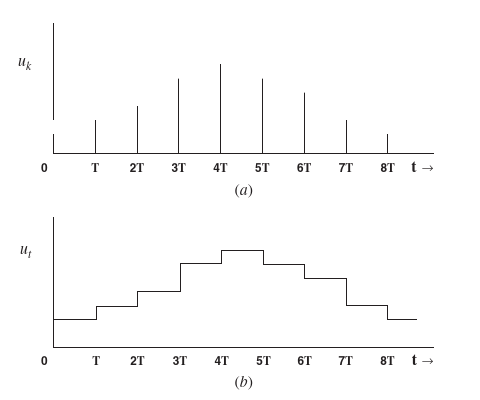
\includegraphics[width=0.5\textwidth, keepaspectratio]{figuras/figure7.2-2.png}\label{fig7.2-2}
    \fonte{\cite{Stevens2016}}
\end{figure}

Evidentemente, as técnicas numéricas introduzem problemas de tratamento bastante complexos, como a questão da estabilidade do método numérico empregado, a estimativa dos erros, bem como os erros introduzidos pela amostragem, quantificação dos sinais, imperfeições dos sensores, ruídos, entre outras. Não obstante, para nosso propósito utilizamos o modelo mais simples possível, ignorando esses problemas até a discussão sobre os resultados, ao final.
